\section{Resultados}
A continuación se presentarán los resultados de los experimentos.

\subsection{Captura de la Facultad}

\begin{figure}[H]
  \centering
    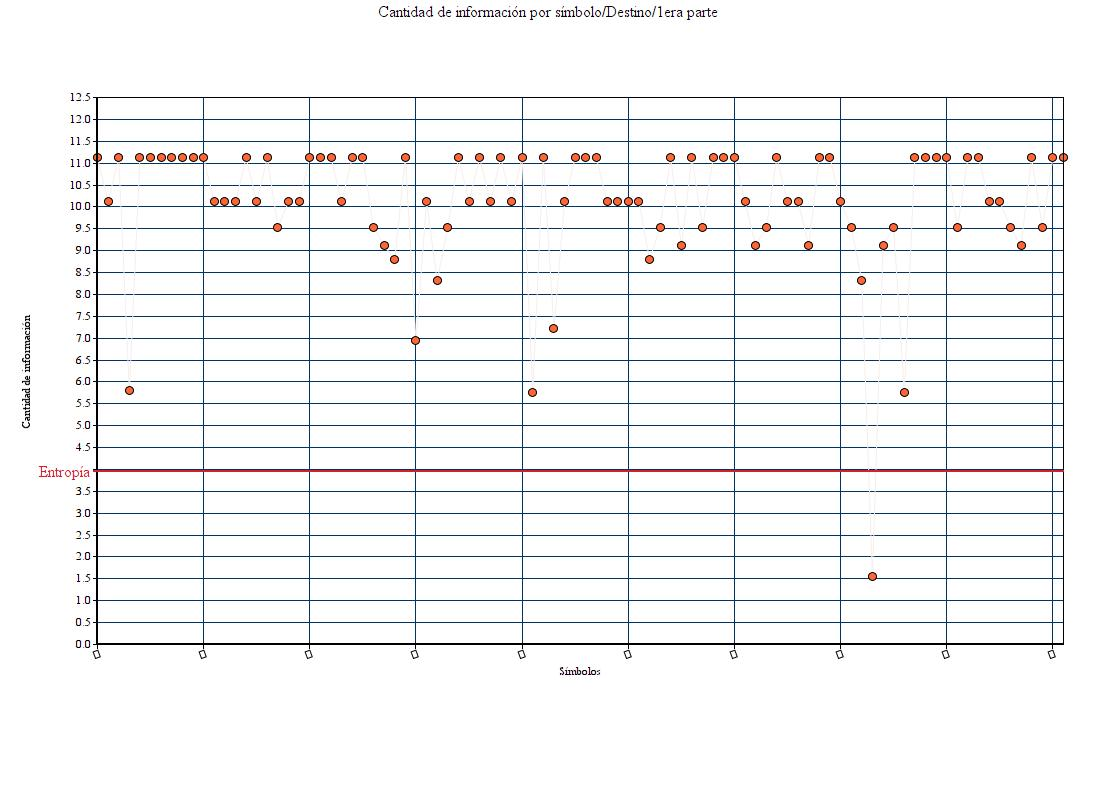
\includegraphics[scale=0.45]{imagenes/graficos/entropiaCantInf/02destino1eraParte.jpg}
  \caption{Cantidad de Información por Símbolo (Destinos) VS Entropía (Parte 1)}
  \label{fig:ejemplo}
\end{figure}
\begin{figure}[H]
  \centering
    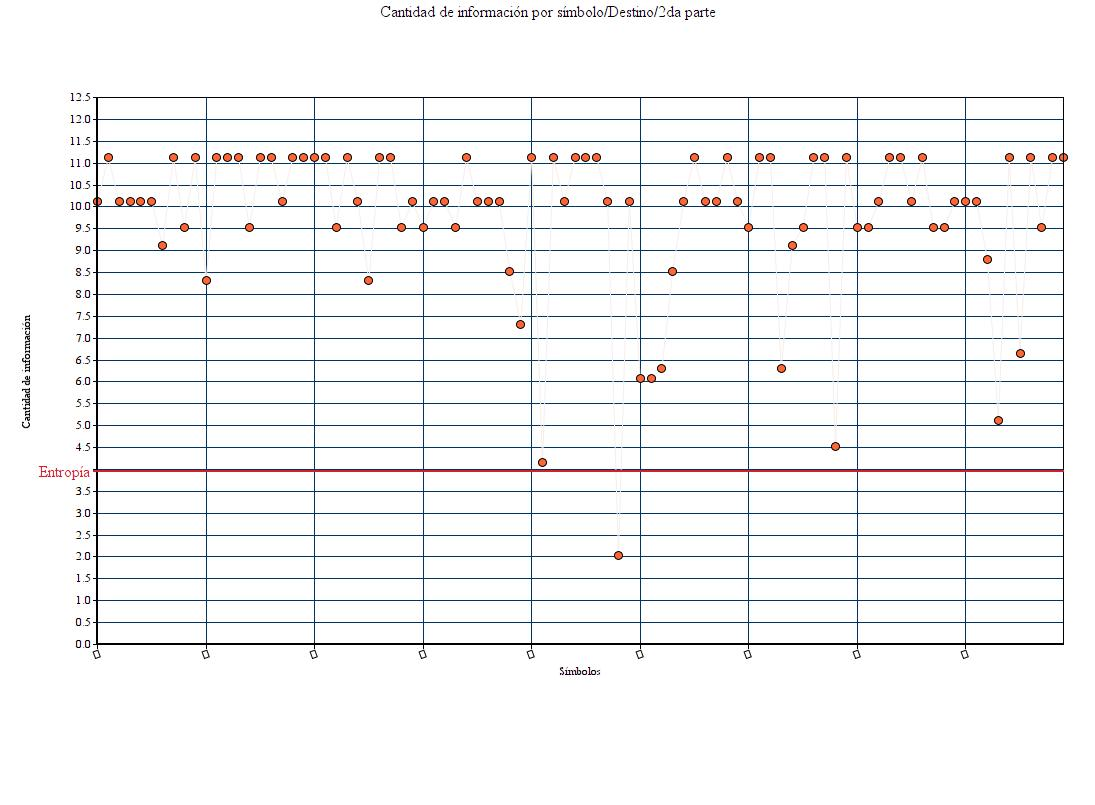
\includegraphics[scale=0.45]{imagenes/graficos/entropiaCantInf/02destino2daParte.jpg}
  \caption{Cantidad de Información por Símbolo (Destinos) VS Entropía (Parte 2)}
  \label{fig:ejemplo}
\end{figure}

En las Figuras 1 y 2, es decir, cuando se tomaron únicamente las direcciones IP de destino en el modelado, se puede ver cómo la mayor parte de los símbolos proveen una gran cantidad de información en contraste con la entropía y también cómo una minoría se destaca por proveer muy poca información. En cambio en las Figuras 3 y 4, donde se consideraron sólo las direcciones origen, si bien ocurre algo similar a lo anterior, es un poco menos acentuada la diferencia.

\begin{figure}[H]
  \centering
    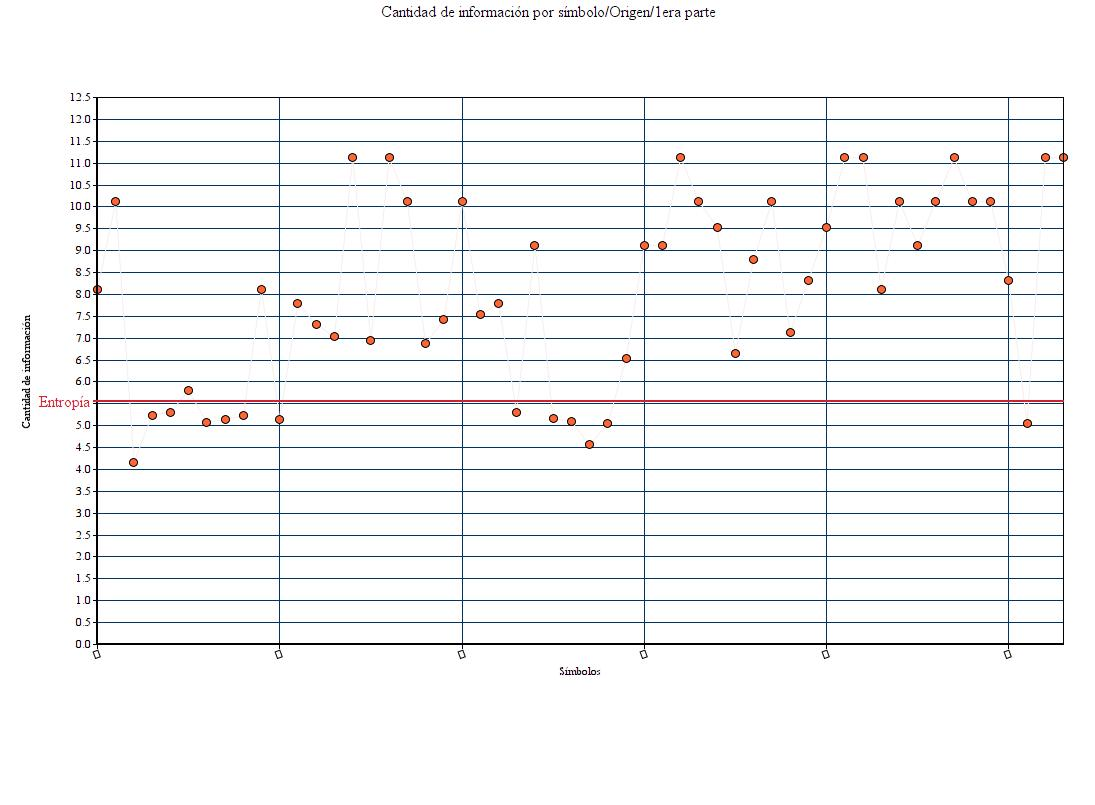
\includegraphics[scale=0.45]{imagenes/graficos/entropiaCantInf/02origen1eraParte.jpg}
  \caption{Cantidad de Información por Símbolo (Orígenes) VS Entropía (Parte 1)}
  \label{fig:ejemplo}
\end{figure}


\begin{figure}[H]
  \centering
    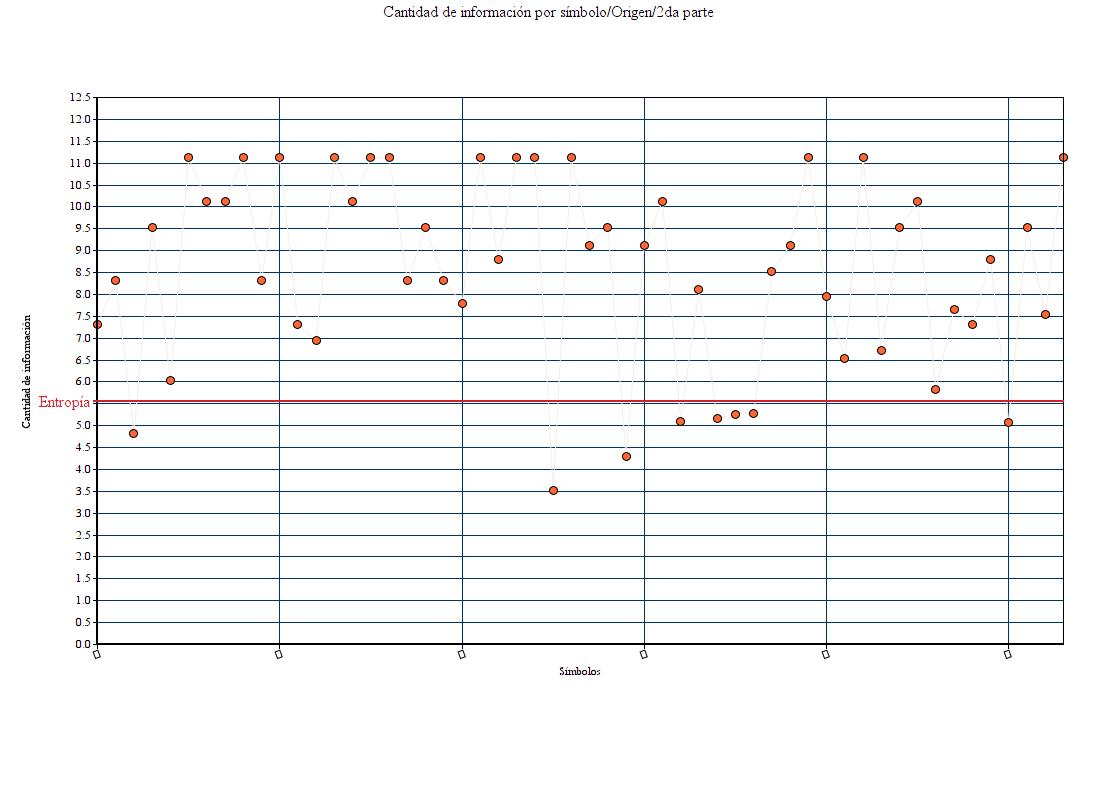
\includegraphics[scale=0.45]{imagenes/graficos/entropiaCantInf/02origen2daParte.jpg}
  \caption{Cantidad de Información por Símbolo (Orígenes) VS Entropía (Parte 2)}
  \label{fig:ejemplo}
\end{figure}

\newpage

\begin{figure}[H]
  \centering
    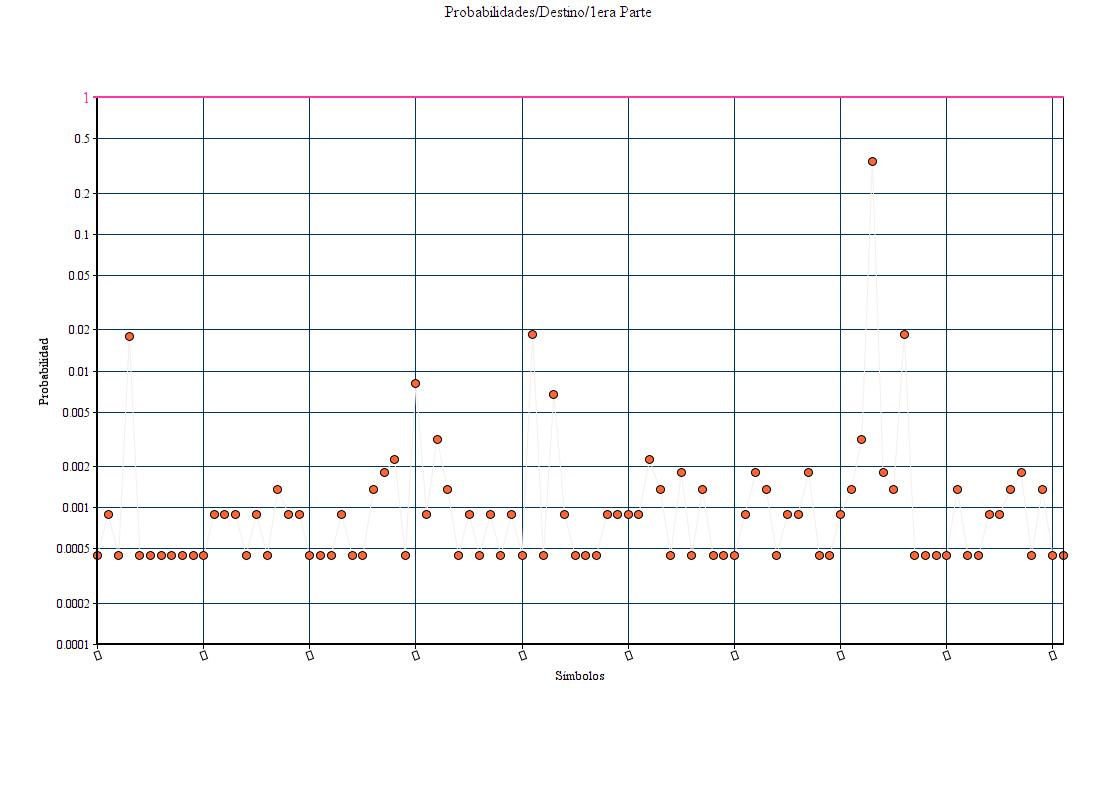
\includegraphics[scale=0.45]{imagenes/graficos/Probabilidades/02destino1eraParte.jpg}
  \caption{Probabilidad de cada Símbolo (Destinos) VS Entropía (Parte 1)}
  \label{fig:ejemplo}
\end{figure}

\begin{figure}[H]
  \centering
    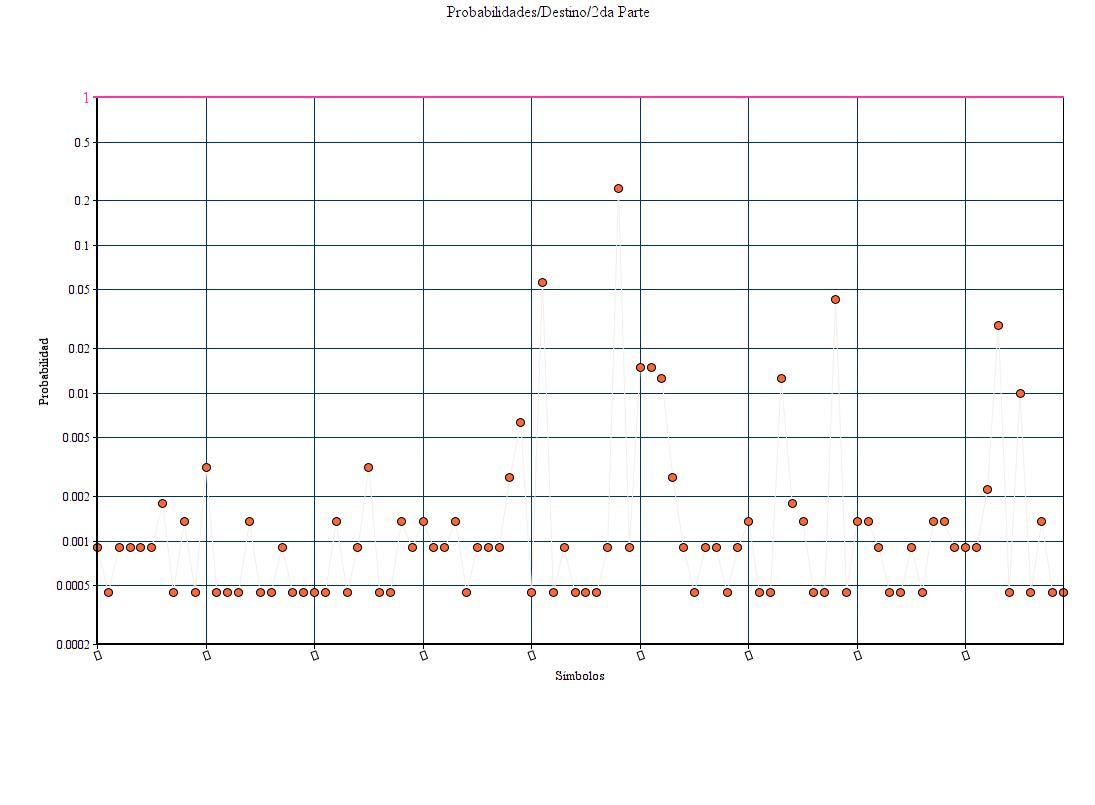
\includegraphics[scale=0.45]{imagenes/graficos/Probabilidades/02destino2daParte.jpg}
  \caption{Probabilidad de cada Símbolo (Destinos) VS Entropía (Parte 2)}
  \label{fig:ejemplo}
\end{figure}

\newpage

En el caso de las probabilidades por símbolo ocurre algo análogo a lo que pasaba con la cantidad de información por símbolo, es decir, para los destinos la mayoría tienen una probabilidad muy baja salvo unos pocos que destacan por tener una alta probabilidad, y con los orígenes se presenta algo muy similar pero con las probabilidades un poco más dispersas y no tan marcada la diferencia.

\begin{figure}[H]
  \centering
    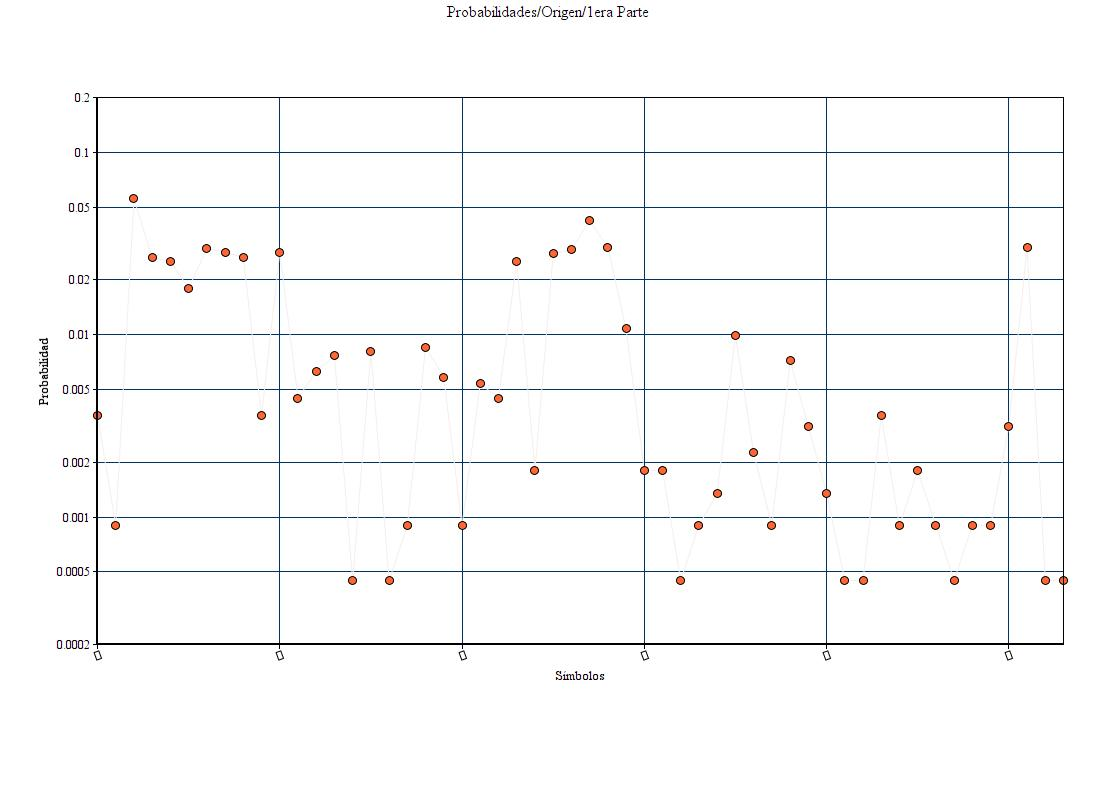
\includegraphics[scale=0.45]{imagenes/graficos/Probabilidades/02origen1eraParte.jpg}
  \caption{Probabilidad de cada Símbolo (Orígenes) VS Entropía (Parte 1)}
  \label{fig:ejemplo}
\end{figure}

\begin{figure}[H]
  \centering
    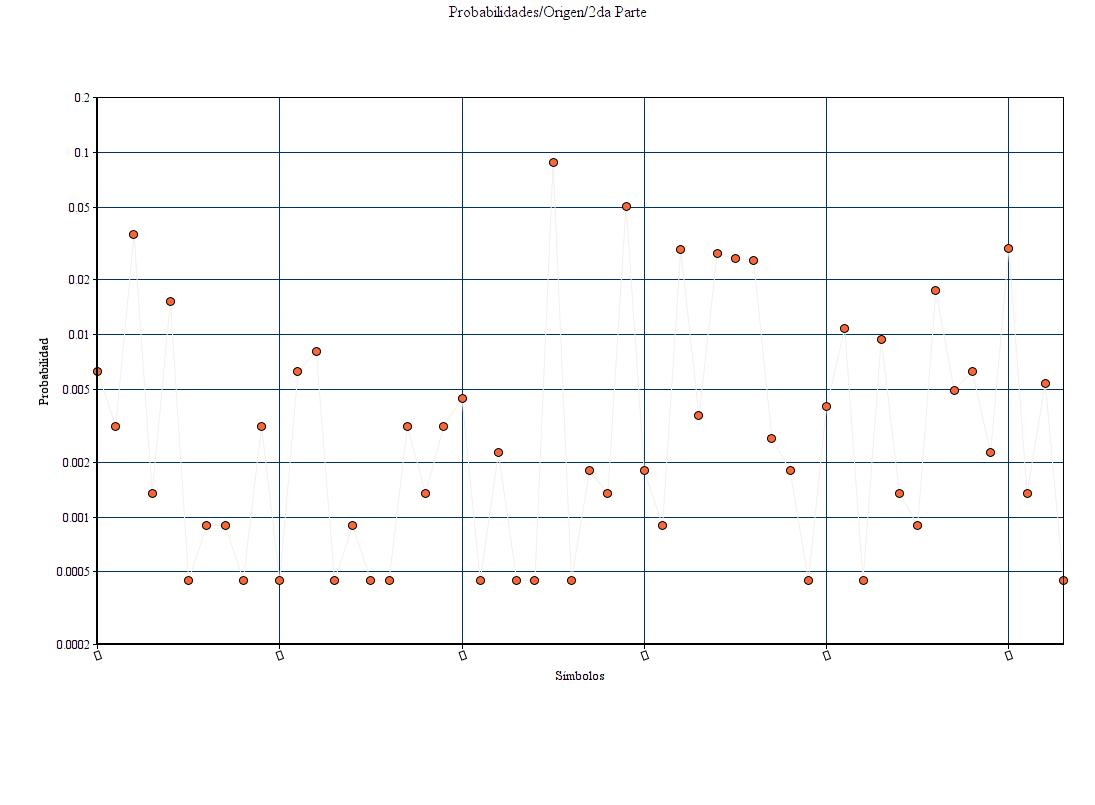
\includegraphics[scale=0.45]{imagenes/graficos/Probabilidades/02origen2daParte.jpg}
  \caption{Probabilidad de cada Símbolo (Orígenes) VS Entropía (Parte 2)}
  \label{fig:ejemplo}
\end{figure}

\begin{figure}[H]
  \centering
    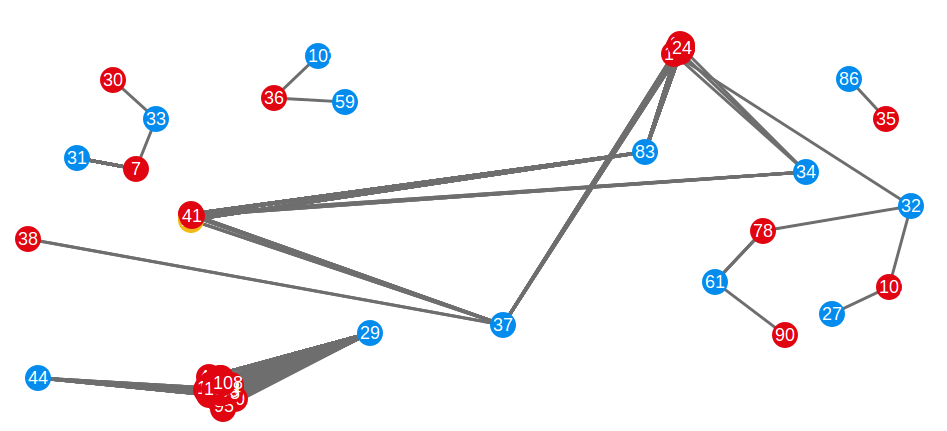
\includegraphics[scale=0.6]{imagenes/graficos/grafos/facultad.png}
  \caption{Red de conexiones entre nodos}
  \label{fig:ejemplo}
\end{figure}

Y ACÁ VA EL CHAMUYO SOBRE EL GRAFO DE LA FACULTAD Y HAY QUE MEJORAR EL CAPTION SEGURO O SACÁRSELO.

\newpage
\subsection{Captura de Starbucks}

\begin{figure}[H]
  \centering
    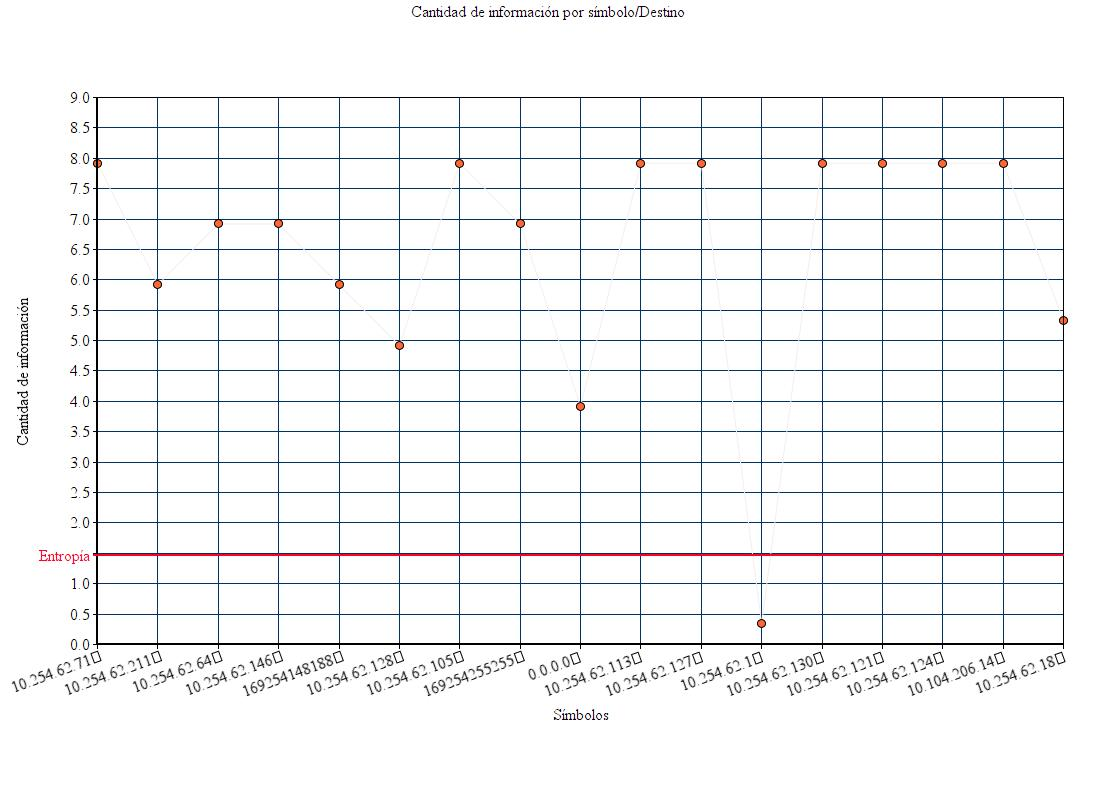
\includegraphics[scale=0.45]{imagenes/graficos/entropiaCantInf/04destino.jpg}
  \caption{Cantidad de Información por Símbolo (Destinos) VS Entropía}
  \label{fig:ejemplo}
\end{figure}

\begin{figure}[H]
  \centering
    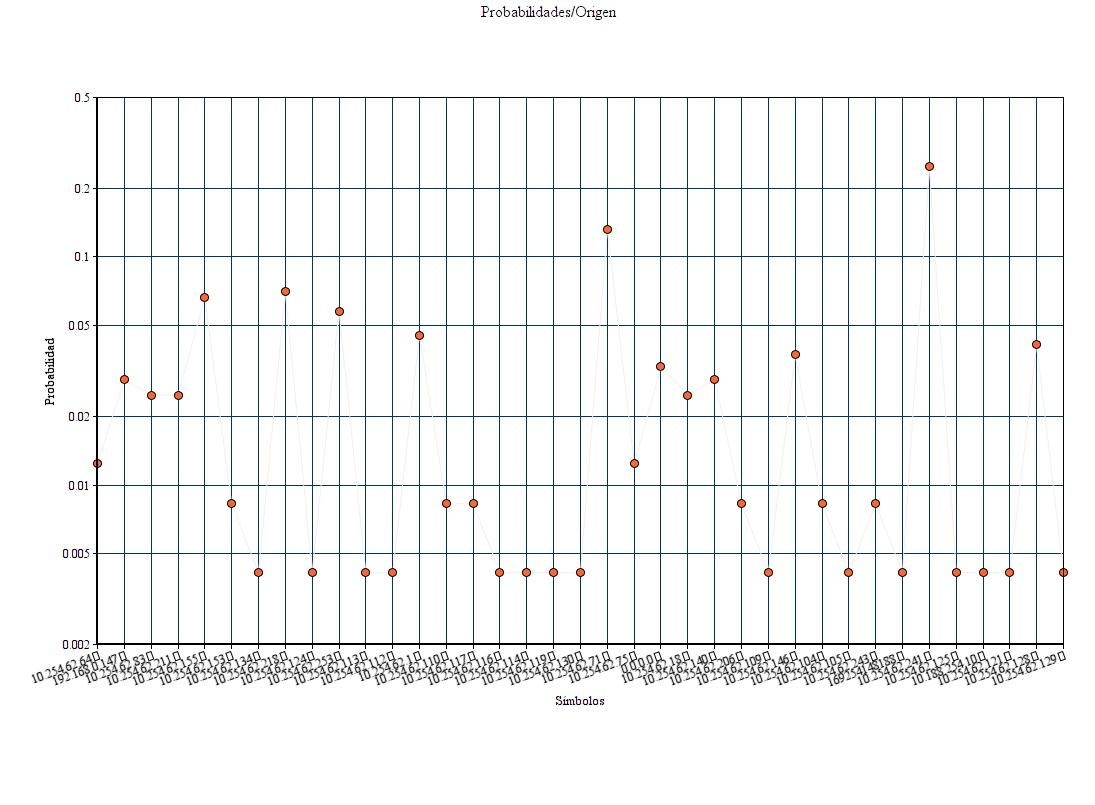
\includegraphics[scale=0.45]{imagenes/graficos/entropiaCantInf/04origen.jpg}
  \caption{Cantidad de Información por Símbolo (Orígenes) VS Entropía}
  \label{fig:ejemplo}
\end{figure}

